\documentclass[11pt,letterpaper]{article}

%\usepackage{fontspec}
%\usepackage[utf8]{inputenc}
\usepackage{textcomp,marvosym}
\usepackage{amsmath,amssymb}
\usepackage[normalem]{ulem}
\usepackage[left]{lineno}
\usepackage{booktabs}
\usepackage{changepage}
\usepackage{rotating}
\usepackage{color}
\usepackage{natbib}
\usepackage{setspace}
\usepackage{array}
\usepackage{fancyhdr}
\usepackage{graphicx}
\usepackage{xspace}
\usepackage[hidelinks]{hyperref}
\urlstyle{same}
\usepackage{threeparttable}
\doublespacing

% make index - for this to work, the .tex file needs to be in the root directory
\usepackage{imakeidx}
\makeindex[columns=2, title=Index]

\raggedright
\textwidth = 6.5 in
\textheight = 8.25 in
\oddsidemargin = 0.0 in
\evensidemargin = 0.0 in
\topmargin = 0.0 in
\headheight = 0.0 in
\headsep = 0.5 in
\parskip = 0.1 in
\parindent = 0.2in

% Bold the 'Figure #' in the caption and separate it from the title/caption with a period
% Captions will be left justified
\usepackage[aboveskip=1pt,labelfont=bf,labelsep=period,justification=raggedright,singlelinecheck=off,font=small]{caption}

% Remove brackets from numbering in List of References
%\makeatletter
%\renewcommand{\@biblabel}[1]{\quad#1.}
%\makeatother

% Self defined commands
\newcommand{\degC}{$^{\circ}$C\xspace}
\newcommand{\dC}{$\delta^{13}$C\xspace}
\newcommand{\dO}{$\delta^{18}$O\xspace}
\newcommand{\SrSr}{$^{87}$Sr/$^{86}$Sr\xspace}
\newcommand{\permil}{\textperthousand\xspace}
\newcommand{\dsil}{$d$\xspace}
\newcommand{\UPb}{$^{206}$Pb/$^{238}$U\xspace}
%

\pagestyle{myheadings}
\pagestyle{fancy}
\fancyhf{}
\lhead{Park et al., accepted for publication in the AGU book entitled \textit{Environmental Change and large igneous provinces: The Deadly Kiss of LIPs}}
\rhead{\thepage}

\begin{document}

\begin{flushleft}
{\Large \textbf{Evaluating the relationship between the area and latitude of large igneous provinces and Earth's long-term climate state}}

Yuem Park\textsuperscript{1},
Nicholas L. Swanson-Hysell\textsuperscript{1},
Lorraine E. Lisiecki\textsuperscript{2},
Francis A. Macdonald\textsuperscript{2}

\bigskip
\textsuperscript{1} Department of Earth and Planetary Science, University of California, Berkeley, CA, USA

\textsuperscript{2} Department of Earth Science, University of California, Santa Barbara, CA, USA
\bigskip

\end{flushleft}

\noindent\textit{This article is accepted for publication in the AGU book entitled \textit{Environmental Change and large igneous provinces: The Deadly Kiss of LIPs}.}

\linenumbers

\section*{ABSTRACT \label{sec:ABSTRACT}}

One of the hypothesized effects of large igneous provinces (LIPs) is planetary cooling\index{cooling} on million-year timescales associated with enhanced silicate weathering\index{silicate weathering} of the freshly-emplaced basalt\index{basalt}. This study combines reconstructions of the original surface extent and emplacement ages of LIPs, a paleogeographic model, and a parameterization of LIP erosion to estimate LIP area in all latitudinal bands through the Phanerozoic. This analysis reveals no significant correlation between total LIP area, nor LIP area in the tropics, and the extent of continental ice sheets. The largest peaks in tropical LIP area are at times of non-glacial climate. These results suggest that changes in planetary weatherability associated with LIPs are not the fundamental control on whether Earth is in a glacial or non-glacial climate, although they could provide a secondary modulating effect in conjunction with other processes.

\section*{INTRODUCTION \label{sec:INTRODUCTION}}

Global weatherability is the sum of factors aside from climate itself that contribute to overall global weathering and associated CO$_2$ consumption, such as the latitudinal distribution of continents and mountain belts \citep{Kump1997a}. On a planet with high weatherability, the CO$_2$ input from volcanism can be removed via silicate weathering\index{silicate weathering} at a lower atmospheric CO$_2$ concentration than on a less weatherable planet. Basaltic\index{basalt} regions consume more CO$_2$ than regions where the bedrock composition is closer to bulk continental crust because mafic lithologies have relatively high concentrations of Ca and Mg (that ultimately sequester carbon through precipitation as carbonate), constitute minerals with relatively high reactivity \citep{Gislason2003a}, and have relatively high weathering rates \citep{Dessert2003a, Ibarra2016a}. Furthermore, data from basaltic\index{basalt} watersheds show that chemical weathering rates are highest in regions with high runoff and temperature. As a result, CO$_2$ consumption in basaltic\index{basalt} regions is most pronounced in the tropical rain belt \citep{Dessert2003a, Hartmann2009a, Hartmann2014a}.

One aspect of large igneous province (LIP) emplacement that has been hypothesized to relate to long-term global climate is the effect that associated mafic lithologies could have on increasing global weatherability and driving cooling\index{cooling}. In particular, the emplacement of LIPs in the tropics has been hypothesized to be associated with specific episodes of climatic cooling\index{cooling} on Earth. In the Neoproterozoic, the emplacement of the ca. 720~Ma Franklin LIP in the tropics, in concert with elevated runoff rates associated with supercontinent break-up, has been implicated as a major contributor to the cooling\index{cooling} that initiated the Sturtian `Snowball Earth' \citep{Donnadieu2004b, Macdonald2010a, Cox2016a}. In the Cenozoic, the movement of the Deccan LIP into the tropical rain belt, together with the low-latitude emplacement of the Ethiopian Traps, has been implicated in drawing down CO$_2$ levels in the lead-up to Oligocene glaciation of Antarctica \citep{Kent2008a, Kent2013a}. More recently, \citet{Johansson2018a} used paleogeographic reconstructions to suggest that tropical LIP area correlates with Phanerozoic climate change through comparison with a \textit{p}CO$_{2}$ proxy compilation.

This chapter seeks to address two interconnected questions: 1) how unique are the peaks in low-latitude LIP area that have been proposed to be associated with climatic cooling\index{cooling}?; and 2) how strong is the overall relationship between tropical LIP area and glaciation?

\section*{METHODS}

This study combines reconstructions of the original surface extent and emplacement ages of LIPs, a paleogeographic model, and a parameterization of LIP erosion to estimate LIP area in all latitudinal bands through the Phanerozoic. We then compare these time series of zonal LIP area to the latitudinal extent of continental ice sheets - a proxy for Earth's long term climate state. This study builds upon a zonal LIP area analysis presented in the supplementary materials for \citet{Macdonald2019a} by more rigorously developing parameterizations of LIP erosion and exploring several geologically reasonable LIP post-emplacement scenarios.

Outlines of the original surface extent of continental LIPs through the Phanerozoic (Fig. \ref{fig:LIP_map}) were slightly modified (to ensure that all currently exposed volcanic lithologies are encapsulated by the initial LIP area polygons) from the compilation of \citet{Ernst2017a} and \citet{Ernst2019a}, and emplacement ages were taken from the literature (Table \ref{tab:LIPs}). The LIP original surface extent compilation seeks to reconstruct the original surface extent of LIPs with the caveat that there can be significant uncertainty with doing so, particularly for older more deeply eroded LIPs. These polygons encapsulate all of the preserved rocks associated with a given LIP, including dikes, sills, and layered intrusions, in addition to subaerial volcanics (Fig. \ref{fig:LIP_map}). For some LIPs, this approach may lead to an over-estimate of original surface extent, given that subsurface intrusions could extend over a broader area than the surface volcanics. The polygons also assume complete surface coverage between wide-spread remnants, creating further potential for these original extent outlines to be over-estimates. These original extent outlines could also under-estimate the surface area for some LIPs where flows have been eroded and feeder dikes are not exposed or poorly documented. However, despite these uncertainties, this approach likely provides the best estimates available of original surface extent for ancient LIPs. The extents of presently-exposed volcanics associated with LIPs that were used for present-day area estimates (Fig. \ref{fig:LIP_map}) and the sources that went into the construction of the original extent polygons by \citet{Ernst2017a} and \citet{Ernst2019a} were taken from a number of resources including the PLATES compilation \citep{Coffin2006a} and more recent compilation efforts associated with the LIPs Reconstruction Project (\citealp{Ernst2013a}; Table \ref{tab:LIPs}).

After LIPs are emplaced, they progressively erode. In order to account for the associated decrease in area with time, \citet{Godderis2017a} took the approach of fitting an exponential decay function to estimates of the original surface extent and the current surface extent of 5 LIPs. They used the resulting exponential decay constants to develop a first-order parameterization of changing LIP area through time. We extend this approach to 19 basaltic\index{basalt} LIPs for which there are estimates of the original surface extent of the province and the current surface extent of rocks associated with the province (Fig. \ref{fig:LIP_preservation}). While there are significant uncertainties associated with the area estimates, this compilation suggests that an exponential decay function is an appropriate first-order representation of the progressive reduction in LIP area (Fig. \ref{fig:LIP_preservation}). The best-fit exponential function results in a LIP area half-life of 29~Myr. However, since we explicitly account for LIP burial separately in our area analysis (see below), we exclude from our estimation of a representative LIP area half-life the 6 of 19 LIPs which are inferred to have been partially or completely buried. This latter approach yields a slightly longer best-fit half-life of 36~Myr (Fig. \ref{fig:LIP_preservation}). Although the exponential fit to the 13 unburied LIPs is good (i.e. it yields a low root mean square error of 0.14), if each LIP is fit individually with an exponential decay function, there is variability in the estimated half-lives from $\sim$20~Myr up to $\sim$120~Myr for the Deccan Traps (Table \ref{tab:LIPs}). In the analysis of LIP area through time, we implement decay scenarios informed by these results: the `t$_{1/2}$ = 36~Myr' scenario uses the best-fit half-life of 36~Myr, while the `t$_{1/2}$ = 120~Myr' scenario uses the slower decay. Given that the post-emplacement weathering and erosional history of each LIP should be dependent on the tectonic and climatic setting that each LIP experiences during and after emplacement, this approach is simplistic, but it provides a framework for analysis. The LIP reconstructions used in this study also include pre-Phanerozoic LIPs. However, given the imposed exponential decay since emplacement, the inclusion of these LIPs does not significantly influence the calculated LIP areas through the Phanerozoic, which is the focus of this analysis.

Of the tectonic factors that could alter exposed LIP area, the most consequential is near-immediate burial by sediment of LIP volcanics that are co-located with a rift basin. There are numerous examples in the record where there is partial or complete burial of a LIP associated with rifting and thermal subsidence (Table \ref{tab:LIPs}). For example, the Afar LIP is both associated with the Ethiopian Traps which form plateau flood basalts\index{basalt} as well as successful rifting in the region of the Red Sea that has resulted in burial (Fig. \ref{fig:LIP_map}). To account for the rapid decrease in exposed surface area that would result from burial by sediments in a rift basin, we impose two different burial scenarios for LIPs that are co-located with rifting. The `50\% burial' scenario imposes instantaneous burial of 50$\%$ of the LIP area while the `100\% burial' imposes instantaneous burial of the entire LIP as an end-member scenario. A limitation of our treatment of LIPs that are co-located with rifting is that we `bury' all of these LIPs instantly at the time of emplacement and to the same degree when in fact the degree and timing of burial of these LIPs may vary substantially. The LIP area analysis uses all of the available combinations of the distinct decay and burial scenarios described above. 

Our LIP reconstruction differs from that of \citet{Johansson2018a}. In contrast to the decay and decay+burial scenarios implemented on estimates of original LIP extent in this study, \citet{Johansson2018a} uses a static extent for each LIP throughout the reconstruction. In their analysis, some of the polygons correspond to the present-day surface extent and some represent the original extent that includes currently buried portions of the LIP (e.g. the Keweenawan Midcontinent Rift for which the implemented extent in \citealp{Johansson2018a} is from geophysical data that largely corresponds to buried subsurface exposures).

The original surface extent LIP polygons were assigned a plate ID corresponding to a tectonic unit on Earth using the polygons of \citet{Torsvik2016a} for the Phanerozoic. The LIP polygons and tectonic units were reconstructed from 520~Ma to the present (e.g. Fig. \ref{fig:Reconstruction_Snapshots}) utilizing the paleogeographic model of \citet{Torsvik2016a} in the spin axis reference frame (anchor plate ID of 1). This paleogeographic model was updated to include revisions to Ordovician Laurentia \citep{Swanson-Hysell2017a} and Paleozoic Asia \citep{Domeier2018a}. Reconstructions and area calculations within latitude bands utilized the pyGPlates function library and custom Python scripts. The total LIP area and the LIP area reconstructed within the tropical rain belt were calculated for the various decay and burial scenarios at a resolution of 5~Myr (Fig. \ref{fig:LIP_Areas}B and C). All the data and code necessary to reproduce the analyses and figures presented in this study can be downloaded from GitHub (\url{https://github.com/Swanson-Hysell-Group/2019_large_igneous_provinces}).

The ascent of air near the equator associated with Earth's large-scale Hadley circulation promotes precipitation and leads to a low-latitude band of high rainfall known as the tropical rain belt. In contrast, the descending branches of the Hadley circulation in the subtropics are associated with aridity \citep{Manabe1969a}. We use 15\textdegree~S to 15\textdegree~N as a working definition of the tropical rain belt, as these latitudes approximately correspond with a sharp increase in zonal mean precipitation when approaching the equator to values greater than 1.0~m/yr in modern climatalogical data (\citealp{Kalnay1996a}; Fig. \ref{fig:Climatology}). Other parameters that could be used to define the tropical rain belt are runoff and precipitation minus evaporation (P--E). When approaching the equator in modern climatological data, zonal mean runoff sharply increases to values above 0.25~m/yr between approximately $\pm$10\textdegree\xspace and $\pm$15\textdegree\xspace (\citealp{Fekete1999a}; Fig. \ref{fig:Climatology}), and zonal mean P--E sharply increases to values above 0.5~m/yr also between approximately $\pm$10\textdegree\xspace and $\pm$15\textdegree\xspace (\citealp{Trenberth2011a}; Fig. \ref{fig:Climatology}). While seasonally high precipitation within $\pm$15\textdegree\xspace of the equator associated with migration of the intertropical convergence zone could be a driver of high chemical weathering, annual mean runoff is often the value that is used within parameterizations of chemical weathering (e.g. \citealp{West2012a}). Using runoff or P--E favors a definition of the tropical rain belt that is closer to $\pm$10\textdegree\xspace rather than $\pm$15\textdegree\xspace. Therefore, we tested the sensitivity of our results to the assumed width of the tropical rain belt by performing the tropical LIP area calculations with a tropical rain belt width of $\pm$10\textdegree\xspace. We also calculated the area of LIPs within $\pm$20\textdegree\xspace of the equator (a width that includes part of the arid subtropics) in order to account for uncertainties in the paleolatitude of LIPs in the paleogeographic model. We find that both of these additional analyses (LIP area calculated within $\pm$10\textdegree\xspace and $\pm$20\textdegree\xspace of the equator) yield similar results to those obtained when LIP area is calculated within $\pm$15\textdegree\xspace of the equator (Table \ref{tab:stats}).

In \citet{Evans2006a}, the reconstructed paleolatitudes of basins with thick, basin-wide evaporite deposition are shown to be consistently in the subtropics throughout the Phanerozoic and the Proterozoic, suggesting that the large-scale atmospheric circulation that gives rise to intense precipitation in the tropical rain belt and an arid subtropical climate is stable through time. However, subsequent work by \citet{Boucot2013a} and \citet{Cao2018a} has interpreted evaporite deposits to have formed at or near the equator at times in the Phanerozoic. While some of this variability could be attributed to waxing/waning of the width of the tropical rain belt as a whole, it is important to note that there can be large deviations in local precipitation from the zonal mean due to factors such as monsoon-related precipitation \citep{Trenberth2000a}, or continentality (i.e. how dispersed or amalgamated the continents are) which can lead to aridity in continental interiors. For instance, much of the Early Cretaceous low-latitude evaporite deposits were formed in basins that were located deep within arid continental interiors at the time of deposition \citep{Boucot2013a, Cao2018a}. Furthermore, in contrast to \citet{Evans2006a}, the compilation of evaporite deposits of \citet{Boucot2013a} contains sedimentary sequences in which the occurrence of evaporitic minerals is limited (e.g. to disseminated gypsum pseudomorphs). Such limited evaporitic mineral precipitation could be attributed to seasonal evaporation that transiently led to saturation states that otherwise would not be expected for that latitude. Nevertheless, a limitation of the LIP analysis described in this study is that it does not account for deviations in local precipitation from the zonal mean (due to the infeasibility of running a highly-resolved global climate model at each time-step in the analysis). However, evaporite deposits, including those in which the occurrence of evaporitic minerals is limited, are distributed bimodally about the equator in the subtropics for the vast majority of the past $\sim$420~Myr \citep{Cao2018a} and overall stability of the large-scale atmospheric circulation is predicted by climate dynamics \citep{Donohoe2017a}. Therefore, the assumption of enhanced precipitation and runoff in the tropics throughout the Phanerozoic is warranted.

To evaluate the relationship between Earth's climate state and total and tropical LIP area, we compared these areas to a compilation of the latitudinal extent of continental ice sheets over the Phanerozoic (\citealp{Macdonald2019a}; Fig. \ref{fig:LIP_Areas}E). The goal in doing so is to evaluate the hypothesis that there is a correlation between LIP area in the tropics and Earth's long-term climate state. The land ice record is an imperfect tracker of climate as it is insensitive to changes in temperature during non-glacial intervals, is influenced by additional factors such as the physical geography of the continents during glacial intervals, and is potentially vulnerable to removal from the observable geologic record via erosion and burial. Furthermore, the threshold \textit{p}CO$_2$ for establishing a glacial climate is dependent on ocean circulation and changing solar luminosity (e.g. \citealp{Shevenell2004a, DeConto2008a}). Nevertheless, it forms a physical record of Earth's climate through time and delineates glacial and non-glacial climate states. We take two approaches for comparison between the LIP area reconstructions and the record of ice extent. The first is to calculate the Pearson correlation coefficient between LIP area and the extent of ice away from the pole. The second is to consider the degree of overlap between intervals of high LIP area (defined as LIP area \textgreater30\% of the maximum in a given post-emplacement model) and intervals of glacial climate (defined as ice extent \textgreater10\textdegree\xspace from the poles). This overlap approach places less emphasis on the specific magnitudes of the peaks in the compiled ice extent and LIP area records.

Another approach would be to compare the LIP area reconstructions to proxy compilations of \textit{p}CO$_2$ (as done by \citealp{Johansson2018a}) instead of the latitudinal extent of continental ice sheets. However, such \textit{p}CO$_2$ proxies are potentially problematic as they can be difficult to calibrate in deep time and can be affected by secondary alteration. Even when stringent quality criteria and the latest understanding of each of the \textit{p}CO$_2$ proxies have been applied to available \textit{p}CO$_2$ records \citep{Foster2017a}, both significant uncertainty in the estimated \textit{p}CO$_2$ for any given data point as well as disagreement between techniques remain (Fig. \ref{fig:LIP_Areas}E). For instance, in the Late Triassic ($\sim$240-200~Ma), estimates of \textit{p}CO$_2$ span $\sim$3000~ppm. Even a probabilistic approach to a large \textit{p}CO$_2$ proxy data set can not constrain \textit{p}CO$_2$ at the 95\% confidence level to within a few hundred ppm for any given time interval, especially when we look deeper in time than the Cenozoic (\citealp{Foster2017a}; Fig. \ref{fig:LIP_Areas}E). For the pedogenic carbonate \dC proxy, which forms the majority of the pre-Cenozoic data in the compilation of \citet{Foster2017a}, such scatter could result from diagenesis \citep{Michel2016a} and the sensitivity of the \textit{p}CO$_2$ estimates on assumptions regarding soil-respired CO$_{2}$ \citep{Montanez2013a}. Nevertheless, despite these shortcomings, the \textit{p}CO$_2$ proxy record is broadly consistent with the ice extent record (Fig. \ref{fig:LIP_Areas}E) - \textit{p}CO$_2$ proxy data decreases $\sim$400-310~Ma as the Late Devonian glacial interval occurs and the Permo-Carboniferous glacial interval begins and waxes, \textit{p}CO$_2$ proxy data roughly increases $\sim$310-240~Ma as the Permo-Carboniferous glacial interval wanes and ends, \textit{p}CO$_2$ proxy data broadly remains relatively high $\sim$240-40~Ma when no glacial intervals are robustly documented, and \textit{p}CO$_2$ proxy data roughly decreases $\sim$40-0~Ma as the Cenozoic glacial interval begins. Given these considerations, we thus prefer to use the latitudinal extent of land ice to reflect Earth's overall climate state throughout the Phanerozoic, despite its own limitations.

\section*{RESULTS}

In the `t$_{1/2}$ = 36~Myr' scenario, we observe four main peaks in the calculated LIP area within the tropics (Fig. \ref{fig:LIP_Areas}C). The first peak ca. 510~Ma is associated with the emplacement of the Kalkarindji LIP, the second peak ca. 380~Ma is associated with the emplacement of the Kola-Dnieper LIP, the third peak ca. 200~Ma is associated with the emplacement of the Central Atlantic Magmatic Province (CAMP), and the fourth peak is associated with both the ca. 30~Ma emplacement of the Afar LIP as well as the earlier drift of the ca. 66~Ma Deccan LIP into the tropics (Figs. \ref{fig:LIP_Areas}A and \ref{fig:Reconstruction_Snapshots}). When we account for burial (`t$_{1/2}$ = 36~Myr + 50\% burial' and `t$_{1/2}$ = 36~Myr + 100\% burial' scenarios), only the latter two of these four peaks are affected -- the ca. 200~Ma peak is attenuated/removed due to the partial/complete burial of the CAMP, and the Cenozoic peak is attenuated due to the partial/complete burial of the Afar LIP. However, after accounting for burial, a minor area of LIPs remain in the tropics from ca. 130~Ma onwards, due to the Equatorial Atlantic Magmatic Province (EQUAMP), Caribbean-Colombian, and Deccan LIPs. Using the longer decay half-life of 120~Myr (the `t$_{1/2}$ = 120~Myr + 100\% burial' scenario) increases the area of LIPs in the tropics at any given time step, and has the effect of extending the duration of each peak.

The only scenario which results in a non-negative Pearson correlation coefficient (0.10) between LIP area in the tropics ($\pm$15\textdegree; Fig. \ref{fig:LIP_Areas}C) and the ice extent record (Fig. \ref{fig:LIP_Areas}E) is the scenario with the slow decay rate and complete burial of LIPs associated with rifting (the `t$_{1/2}$ = 120~Myr + 100\% burial' scenario; Fig. \ref{fig:LIP_correlation}). All other scenarios (including both total LIP area and tropical LIP area) yield a near zero or weak negative correlation coefficient (Fig. \ref{fig:LIP_correlation}). The weak positive correlation of the `t$_{1/2}$ = 120~Myr + 100\% burial' scenario relative to the other scenarios can be primarily attributed to the complete removal of the CAMP, which was emplaced during an extended interval of ice-free conditions, as well as the effect of the longer decay half-life extending the duration of the earlier two peaks, such that they overlap more with the Late Ordovician and Permo-Carboniferous glacial intervals.

To assess the statistical significance of the correlation implied by the Pearson correlation coefficients (or lack thereof), we applied the approach of \citet{Macdonald2019a} and simulated the four glacial episodes (Fig. \ref{fig:LIP_Areas}E) occurring at random times through the past 520~Myr, and recomputed the correlation coefficient and \% overlap between the LIP area in the tropics and the randomly timed glacial intervals for each of these 100,000 simulations (Fig. \ref{fig:LIP_correlation}). This approach accounts for the fact that spurious correlation can arise between auto-correlated data sets such as these, where each value is not independent, but is instead dependent on the previous state of the system. For the `t$_{1/2}$ = 120~Myr + 100\% burial' scenario, 72\% of the randomly timed glacial interval simulations correlate better with LIP area in the tropics than the actual ice extent record. With an associated p-value of 0.72, the null hypothesis that glacial intervals do not correlate to LIP area in the tropics cannot be rejected. Taking this approach, none of the positive or negative correlations that emerge between the LIP area scenarios and the ice extent record are statistically significant (Table \ref{tab:stats}).

\section*{DISCUSSION}

In the original models that proposed the `Fire and Ice' hypothesis as an explanation for the onset of the Sturtian `Snowball Earth' glaciation, chemical weathering was modeled as a function of temperature and runoff only \citep{Donnadieu2004a}. However, such an approach neglects the effects of soil shielding and regolith development in low-relief regions. Recent progress on understanding the relationships between landscapes, topography, and chemical weathering reveals that these effects are important \citep{Gabet2009a, Hartmann2014a, Maher2014a, Godderis2017b}. Soil shielding can lead to a transport-limited weathering regime in which the weathering rate of the underlying bedrock becomes insensitive to kinetic and equilibrium factors such as temperature and runoff - factors that would, in the absence of soil shielding, lead to relatively high weathering rates in the tropical rain belt. As a result, more recent modeling of chemical weathering incorporates such processes and highlights the importance of high-relief regions relative to low-relief ones for setting global weatherability \citep{West2012a, Godderis2017b}. LIPs are often emplaced in relatively low-relief areas, and as such, without active uplift, soil shielding from regolith development on these low-relief LIPs could significantly decrease the local weatherability of a LIP and mute its impact on global weatherability (as suggested in \citealp{Kent2013a}). In this way, soil shielding could explain the lack of correlation between tropical LIP area and ice extent (Figs. \ref{fig:LIP_Areas} and \ref{fig:LIP_correlation}). In contrast, processes that lead to continued exhumation of mafic lithologies and the creation of steep topography that minimizes soil shielding, particularly in tropical regions, may exert a strong control on global weatherability and long-term climate. This interpretation underlies the hypothesis that arc-continent collisions in the tropics during the Ordovician \citep{Swanson-Hysell2017a} and the Cenozoic \citep{Jagoutz2016a} played a significant role in transitions into glacial climate states at those times - a correlation that appears robust throughout the Phanerozoic \citep{Macdonald2019a}.

A complication with the interpretation of soil shielding and limited weathering of LIPs is the rapid area decay rate (t$_{1/2}$ = 36~Myr) inferred from the comparison of current LIP surface extent to estimated original surface extent (Fig. \ref{fig:LIP_preservation}). A couple considerations are relevant with respect to this analysis: 1) the current surface extent of LIP exposure is reduced in part by volcanics being covered by unconsolidated sediments (i.e. regolith development itself) in a number of the provinces; 2) the current surface extent of LIP exposure may be incomplete and an underestimate for some of the provinces; 3) the initial LIP surface extents are typically poorly constrained and are likely over-estimates which could be resulting in inflated interpreted decay rates; and 4) the relationship between LIP area and volume is poorly constrained. Future efforts that improve the LIP database, such as developing better-constrained estimates of original LIP surface extent, constraining burial and uplift histories, and refining the timing of eruptions associated with LIPs, will improve analyses that consider the LIP record in its entirety, such as that in this contribution.

We have focused this analysis on the Phanerozoic record given that well-constrained paleogeographic models are available for the past $\sim$520~Myr. The approach of seeking to evaluate correlation between LIP area and glaciation is further complicated for Neoproterozoic Snowball Earth events because ice-albedo runaway leads to persistent global glaciation on timescales of tens of millions of years without continued forcing through normal carbon cycle processes until sufficient CO$_2$ to drive deglaciation builds up in the absence of silicate weathering\index{silicate weathering} \citep{Hoffman2017a}. Moreover, cooling\index{cooling} past the critical threshold for rapid global glaciation may have occurred on a sub-million year timescale (e.g. \citealp{Macdonald2017a}). Nevertheless, evaluating the hypothesis of tropical LIP area associated with the ca. 720~Ma Franklin LIP increasing global weatherability and contributing to the onset of the Sturtian Snowball Earth is a major motivating driver behind conducting this analysis.

How does the tropical LIP area associated with the Franklin LIP compare to that observed in the Phanerozoic? Using the paleomagnetic pole of \citet{Denyszyn2009a}, we reconstruct the paleolatitude of the Franklin LIP at the time of emplacement, and find that $\sim$99.7\% (or $\sim$2.6~Mm$^{2}$) of the LIP erupted within 15\textdegree\xspace of the equator. This Franklin LIP tropical area at the time of emplacement is approximately equivalent to the Cenozoic peak, and is smaller than the other Phanerozoic peaks (Fig. \ref{fig:LIP_Areas}C). The ca. 1109~Ma Umkondo is another Precambrian LIP that is constrained to have erupted in the tropics, although it is not known to be associated with any glaciation (no glacial deposits are found within the contemporaneous Midcontinent Rift basin; \citealp{Swanson-Hysell2019a}). We reconstruct the paleolatitude of the Umkondo LIP at the time of emplacement using the paleomagnetic pole of \citet{Swanson-Hysell2015b}, and find that effectively all of the LIP (or $\sim$2.0~Mm$^{2}$) erupted within the tropics, an area that is slightly smaller than that estimated for the Franklin LIP (Fig. \ref{fig:LIP_Areas}C).

Together, these results indicate that the Franklin LIP, when compared to Phanerozoic as well as other Precambrian LIPs, did not have a uniquely large area in the tropics. Given that similar (and larger) peaks in tropical LIP area are not associated with the onset of glacial periods, additional processes beyond an increase in weatherability due to LIP area in the tropics must have been at play in the initiation of the Sturtian Snowball Earth. One such process could have been unusually high planetary albedo associated with the low-latitude continental configuration of the supercontinent Rodinia \citep{Kirschvink1992a, Li2008a}. However, our analysis of zonal continental area reveals an almost invariant tropical continental area from $\sim$400~Ma to the present (Fig. \ref{fig:Continent_Areas}) and consequently no significant correlation between tropical continental area and the ice extent record in the Phanerozoic, although it is intriguing that there is a high and rising low-latitude continental area in the Ordovician. Similar to the LIP area analysis, this continental area analysis suggests that a low-latitude continental configuration can not be invoked as the sole driver of planetary cooling\index{cooling}, although it could be a contributing factor. Another potential contributing process for Neoproterozoic cooling\index{cooling} leading up to the Sturtian glaciation is an increase in global weatherability associated with the collision and accretion of arc terranes within the present-day Arabian-Nubian Shield \citep{Park2018a}. Together, a low-latitude continental configuration and abundant arc-continent collisions in the tropics may have led to a cool background climate, and the emplacement of the Franklin LIP may have further increased global weatherability to the point where the ice-albedo runaway could take effect. However, tropical LIP area associated with the Franklin was not uniquely high, and therefore an associated increase in global weatherability was likely not the sole driver of Snowball Earth onset, consistent with the results of the Phanerozoic analysis.

The temporal overlap between Franklin LIP eruptions and the initiation of Sturtian glaciation remains compelling \citep{Macdonald2010a, MacLennan2018a}. This overlap could support arguments that other aspects of LIP emplacement, such as the injection of sulfur aerosols in the stratosphere \citep{Macdonald2017a}, played a role in the initiation of low-latitude glaciation. The temporary effect on albedo of such aerosols is maximized when they are injected into the atmosphere at low-latitudes into a cool background climate and their presence at high concentrations is pre-conditioned on eruption through sedimentary basins hosting evaporite deposits, as could have been the case for the Franklin LIP \citep{Macdonald2017a}. However, in the cases in which such aerosol-driven cooling\index{cooling} does not result in ice-albedo runaway and a Snowball Earth, the climate would return to its background climate state within years \citep{Macdonald2017a}. A contrasting effect is that, on 1~kyr to 1~Myr timescales, LIP emplacement could instead cause transient warming associated with elevated CO$_{2}$ outgassing leading to transiently high \textit{p}CO$_{2}$, as has been argued for the CAMP \citep{Schaller2011a, Schaller2012a}.

The results from this analysis indicate that when the entire LIP database is considered in conjunction with a paleogeographic reconstruction and this parameterization of erosion, there is no significant relationship between total LIP area nor LIP area in the tropics and the extent of continental ice sheets. While this result need not imply that there is no increase in global weatherability from the emplacement of LIPs, it does suggest that changes in planetary weatherability associated with LIPs are not the fundamental control on whether Earth is in a glacial or non-glacial climate state.

\section*{ACKNOWLEDGEMENTS \label{sec:ACKNOWLEDGEMENTS}}

Richard Ernst provided GIS compilations of LIP extent and present-day exposure that were essential to the analysis. Discussions with Yves Godd\'eris made possible through the France-Berkeley Fund contributed valuably to aspects of the interpretation. Park was supported by NSF Grant 1547434 awarded to Swanson-Hysell.

\clearpage
\newpage

\section*{TABLES}

\begin{table}[h!]
\scriptsize
\caption{Phanerozoic large igneous provinces (and the Franklin).}
\resizebox{\textwidth}{!}{
\begin{tabular}{lc>{\raggedright}p{4cm}cc>{\raggedright}p{4cm}ccl}
\toprule
\textbf{name} & \textbf{age} & \textbf{age ref.} & \textbf{original$^{1}$} & \textbf{present$^{2}$} & \textbf{present area ref.} & \textbf{present/$^{3}$} & \textbf{half-life}$^{4}$ & \textbf{buried?} \\
 & \textbf{(Ma)} & & \textbf{area} & \textbf{area} & & \textbf{original} & \textbf{(Myr)} & \\
 & & & \textbf{(Mm$^{2}$)} & \textbf{(Mm$^{2}$)} & & & & \\
\midrule
Columbia River & 16 & \cite{Kasbohm2018a} & 0.68 & 0.38 & \cite{Buchan2004a} & 0.56 & 19.2 & no \\
 & & & & & & & & \\
Afar & 30 & \cite{Courtillot2003a} & 2.05 & 0.63 & \cite{Coffin2006a} & 0.31 & 17.7 & partial \\
 & & & & & & & & \\
NAIP & 62 & \cite{Larsen2015a} & 1.07 & 0.29 & \cite{Buchan2004a, Coffin2006a} & 0.27 & 33.0 & partial \\
 & & & & & & & & \\
Deccan & 66 & \cite{Schoene2014a} & 0.83 & 0.56 & \cite{Coffin2006a} & 0.68 & 116.6 & no \\
 & & & & & & & & \\
Seychelles & 66 & \cite{Schoene2014a} & 0.46 & 0.00 & \cite{Coffin2006a} & 0.00 & 0.0 & yes \\
 & & & & & & & & \\
Madagascar & 90 & \cite{Cucciniello2010a} & 0.63 & 0.03 & \cite{Coffin2006a} & 0.05 & 20.8 & no \\
 & & & & & & & & \\
Caribbean-Colombian & 94 & \cite{Loewen2013a} & 0.71 & 0.13 & \cite{Coffin2006a} & 0.18 & 37.6 & no \\
 & & & & & & & & \\
HALIP & 95 & \cite{Kingsbury2018a} & 3.60 & 0.15 & \cite{Hartmann2012a} & 0.04 & 20.7 & no \\
 & & & & & & & & \\
EQUAMP & 131 & \cite{Hollanda2016a} & 0.66 & 0.01 & \cite{Hollanda2016a} & 0.01 & 20.5 & no \\
 & & & & & & & & \\
Comei & 132 & \cite{Zhu2009a} & 0.11 & - & - & - & - & no \\
 & & & & & & & & \\
Bunbury & 132 & \cite{Zhu2009a} & 0.03 & 0.00 & \cite{Thorne2014a} & 0.05 & 30.9 & no \\
 & & & & & & & & \\
Parana-Etendeka & 135 & \cite{Florisbal2014a, Almeida2018a} & 3.12 & 0.40 & \cite{Coffin2006a} & 0.13 & 45.7 & partial \\
 & & & & & & & & \\
Trap & 140 & \cite{Ernst2001a} & 0.03 & 0.00 & \cite{Ernst2001a} & 0.00 & 0.0 & no \\
 & & & & & & & & \\
NW Australia Margin & 160 & \cite{Pirajno2012a} & 0.62 & 0.00 & \cite{Coffin2006a} & 0.00 & 0.0 & yes \\
 & & & & & & & & \\
Karoo & 183 & \cite{Burgess2015a} & 3.21 & 0.15 & de Kock compilation$^{5}$ & 0.05 & 41.3 & no \\
 & & & & & & & & \\
Ferrar & 183 & \cite{Burgess2015a} & 0.18 & - & - & - & - & no \\
 & & & & & & & & \\
CAMP & 201 & \cite{Blackburn2013a} & 11.46 & 0.23 & Marzoli and Parisio compilation$^{6}$ & 0.02 & 35.7 & partial \\
 & & & & & & & & \\
Siberia & 252 & \cite{Burgess2015b} & 3.46 & 0.47 & \cite{Coffin2006a} & 0.14 & 87.5 & no \\
 & & & & & & & & \\
Emeishan & 259 & \cite{Zhou2002a} & 0.71 & 0.06 & \cite{Coffin2006a} & 0.09 & 72.9 & no \\
 & & & & & & & & \\
Panjal-Qiangtang & 283 & \cite{Zhai2013a} & 0.11 & - & - & - & - & no \\
 & & & & & & & & \\
Tarim & 290 & \cite{Xu2014a} & 0.35 & - & - & - & - & no \\
 & & & & & & & & \\
Magdalen & 360 & \cite{Murphy1999a} & 0.42 & - & - & - & - & no \\
 & & & & & & & & \\
Vilyui & 374 & \cite{Ricci2013a} & 1.14 & - & - & - & - & no \\
 & & & & & & & & \\
Kola-Dnieper & 380 & \cite{Arzamastsev2014a} & 5.90 & - & - & - & - & no \\
 & & & & & & & & \\
Suordakh & 450 & \cite{Khudoley2013a} & 0.02 & - & - & - & - & no \\
 & & & & & & & & \\
Kalkarindji & 511 & \cite{Jourdan2014a} & 3.54 & 0.17 & \cite{Thorne2014a} & 0.05 & 116.3 & no \\
 & & & & & & & & \\
Franklin & 720 & \cite{Denyszyn2009a} & 2.62 & 0.04 & \cite{Buchan2004a} & 0.02 & 121.8 & no \\
\bottomrule
\end{tabular}
}
\begin{tablenotes}[para,flushleft]
\vspace{0.15cm}
$^{1}$obtained via calculating the area of the continental portions of polygons within the LIP original surface extent compilation of \citet{Ernst2017a} and \citet{Ernst2019a}, shown as blue polygons in Fig. \ref{fig:LIP_map}.
\vspace{0.15cm}

$^{2}$obtained via calculating the area of polygons from the noted reference of presently-exposed volcanics associated with LIPs, shown as orange polygons in Fig. \ref{fig:LIP_map}.
\vspace{0.15cm}

$^{3}$present area / original area
\vspace{0.15cm}

$^{4}$assuming exponential decay with form $N(t) = 2^{t/t_{1/2}}$.
\vspace{0.15cm}

$^{5}$from ArcGIS compilation produced by M. de Kock for the LIPs Reconstruction Project \citep{Ernst2013a}.
\vspace{0.15cm}

$^{6}$from ArcGIS compilation produced by A. Marzoli and L. Parisio for the LIPs Reconstruction Project \citep{Ernst2013a}.
\end{tablenotes}
\label{tab:LIPs}
\end{table}

\begin{table}[h!]
\scriptsize
\caption{Statistics of correlation between large igneous province area and ice extent.}
\resizebox{\textwidth}{!}{
\begin{tabular}{>{\raggedright}p{2.5cm}|cccc|cccc|cccc|cccc}
\toprule
\textbf{} & \multicolumn{4}{c|}{\textbf{within tropics $\pm$15$^{\circ}$}} & \multicolumn{4}{c|}{\textbf{total}$^{5}$} & \multicolumn{4}{c|}{\textbf{within tropics $\pm$10$^{\circ}$}} & \multicolumn{4}{c}{\textbf{within tropics $\pm$20$^{\circ}$}} \\
&&&&&&&&&&&&&&&& \\
\textbf{} & \multicolumn{2}{c}{\textbf{correlation}$^{1}$} & \multicolumn{2}{c|}{\textbf{\% overlap}$^{2}$} & \multicolumn{2}{c}{\textbf{correlation}} & \multicolumn{2}{c|}{\textbf{\% overlap}} & \multicolumn{2}{c}{\textbf{correlation}} & \multicolumn{2}{c|}{\textbf{\% overlap}} & \multicolumn{2}{c}{\textbf{correlation}} & \multicolumn{2}{c}{\textbf{\% overlap}} \\
\textbf{scenario} & \textbf{val.}$^{3}$ & \textbf{p-val.}$^{4}$ & \textbf{val.} & \textbf{p-val.} & \textbf{val.} & \textbf{p-val.} & \textbf{val.} & \textbf{p-val.} & \textbf{val.} & \textbf{p-val.} & \textbf{val.} & \textbf{p-val.} & \textbf{val.} & \textbf{p-val.} & \textbf{val.} & \textbf{p-val.} \\
\midrule
t$_{1/2}$ = 36~Myr & -0.19 & 0.81 & 13 & 0.94 & -0.26 & 0.85 & 30 & 0.95 & -0.22 & 0.86 & 13 & 0.95 & -0.17 & 0.77 & 9 & 0.96 \\
&&&&&&&&&&&&&&&& \\
t$_{1/2}$ = 36~Myr + 50\% burial & -0.14 & 0.73 & 22 & 0.85 & -0.25 & 0.84 & 52 & 0.97 & -0.17 & 0.79 & 9 & 0.90 & -0.10 & 0.67 & 26 & 0.86 \\
&&&&&&&&&&&&&&&& \\
t$_{1/2}$ = 36~Myr + 100\% burial & -0.02 & 0.45 & 22 & 0.65 & -0.14 & 0.74 & 65 & 0.94 & -0.08 & 0.54 & 9 & 0.76 & 0.04 & 0.37 & 22 & 0.65 \\
&&&&&&&&&&&&&&&& \\
t$_{1/2}$ = 120~Myr + 100\% burial & 0.10 & 0.32 & 35 & 0.72 & 0.00 & 0.51 & 100 & 1.00 & 0.02 & 0.40 & 26 & 0.77 & 0.19 & 0.24 & 48 & 0.66 \\
\bottomrule
\end{tabular}
}
\begin{tablenotes}[para,flushleft]
\vspace{0.15cm}
$^{1}$Pearson correlation coefficient between LIP area and the actual ice extent record.
\vspace{0.15cm}

$^{2}$\% of time when both LIP area is \textgreater30\% of the maximum and ice extent is \textgreater10\textdegree\xspace from the poles.
\vspace{0.15cm}

$^{3}$`val.' refers to the computed correlation coefficient/\% overlap between LIP area and the actual ice extent record.
\vspace{0.15cm}

$^{4}$`p-val.' refers to the fraction of randomly timed glacial interval simulations that correlate/overlap better with LIP area than the actual ice extent record (i.e. the p-value with respect to the null hypothesis of no correlation/overlap). P-values \textless0.05 indicate that we can reject the null hypothesis at the 95\% confidence level.
\vspace{0.15cm}

$^{5}$all latitudes.
\end{tablenotes}
\label{tab:stats}
\end{table}

\clearpage
\newpage

\section*{FIGURES}

\begin{figure}[h!]
\begin{center}
	\includegraphics[width=\textwidth]{./Manuscript/Figures/LIP_Map.pdf}
	\caption{Map of current surface extent of volcanic lithologies associated with LIPs that erupted between 520~Ma and the present, as well as the estimates of the initial LIP surface extent used in the area analysis (modified slightly from \citealp{Ernst2017a} and \citealp{Ernst2019a} to ensure that all currently exposed volcanic lithologies are encapsulated by the initial LIP surface area polygons).}
	\label{fig:LIP_map}
\end{center}
\end{figure}

\begin{figure}[h!]
\begin{center}
	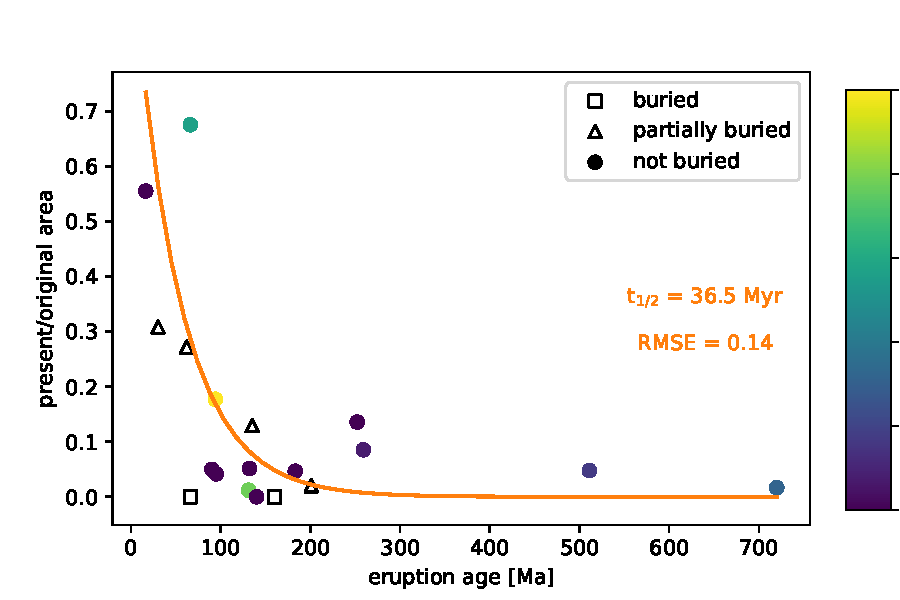
\includegraphics[width=0.6\textwidth]{./Manuscript/Figures/LIP_Preservation.pdf}
	\caption{LIP erosion through time. The ratio of estimates of the present-day surface area to that of the original surface area are shown for 19 basaltic LIPs. An exponential fit is made to the 13 basaltic LIPs that are interpreted to not have been buried after emplacement (Table \ref{tab:LIPs}), which yields a half-life of $\sim$36~Myr. RMSE = root mean square error.}
	\label{fig:LIP_preservation}
\end{center}
\end{figure}

\begin{figure}[h!]
\begin{center}
	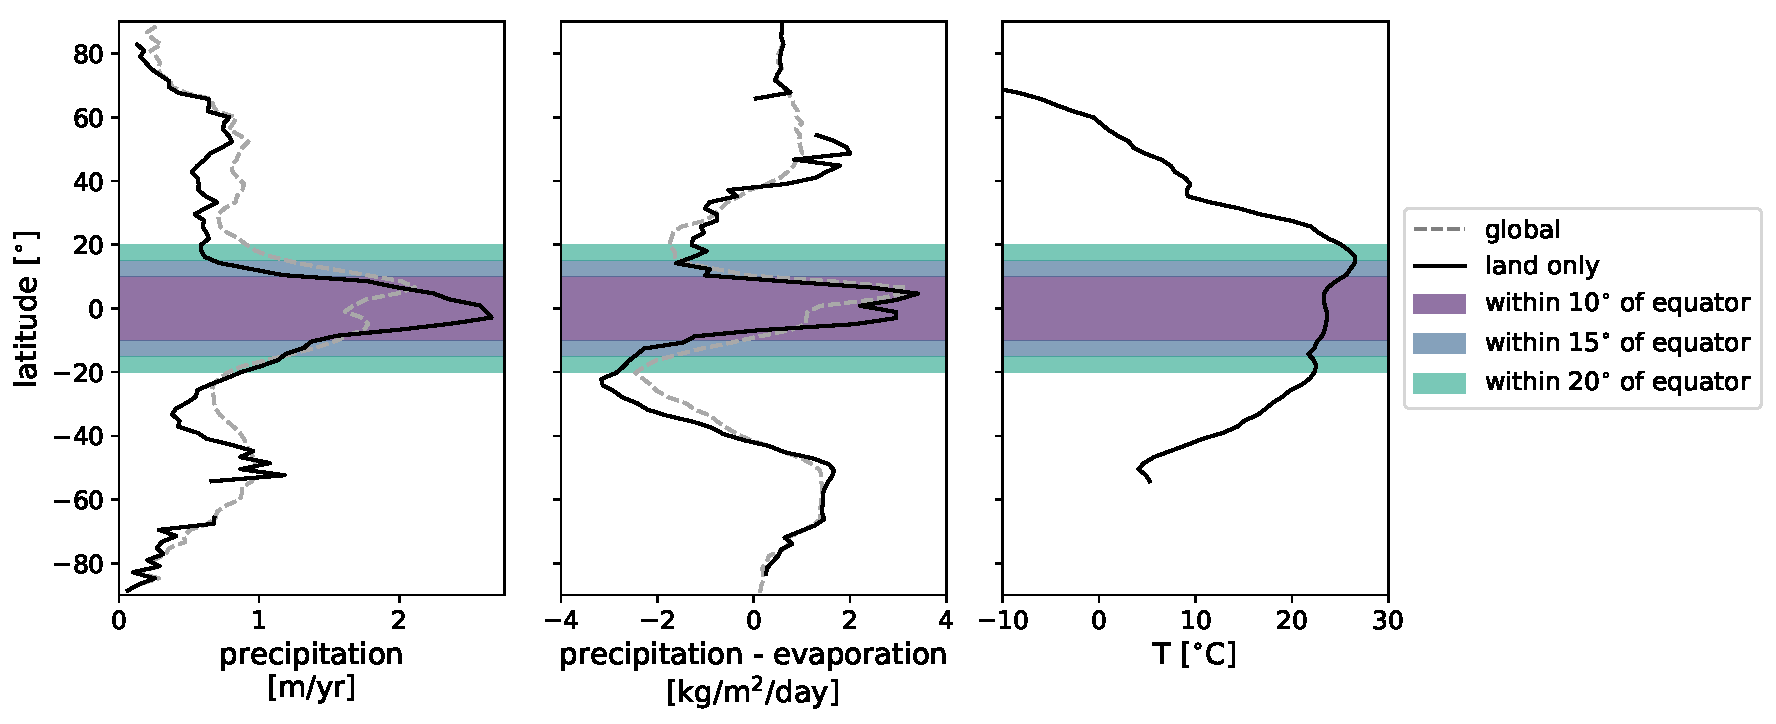
\includegraphics[width=\textwidth]{./Manuscript/Figures/Climatology.pdf}
	\caption{Zonally averaged modern climatological data used to define the tropical rain belt. The global precipitation \citep{Kalnay1996a} and precipitation minus evaporation \citep{Trenberth2011a} data include land and ocean pixels, global temperature data \citep{Kalnay1996a} are from land only, and runoff data \citep{Fekete1999a} are from land only excluding Antarctica. The peak in runoff $\sim$-50\textdegree\xspace is due to anomalously high orographically-induced runoff in the southern Andes, which represents almost all of the land in that latitude belt. Temperature data for Antarctica are off scale. Precipitation, precipitation minus evaporation, and runoff all increase sharply between $\pm$10\textdegree\xspace and $\pm$15\textdegree\xspace.}
	\label{fig:Climatology}
\end{center}
\end{figure}

\begin{figure}[h!]
\begin{center}
	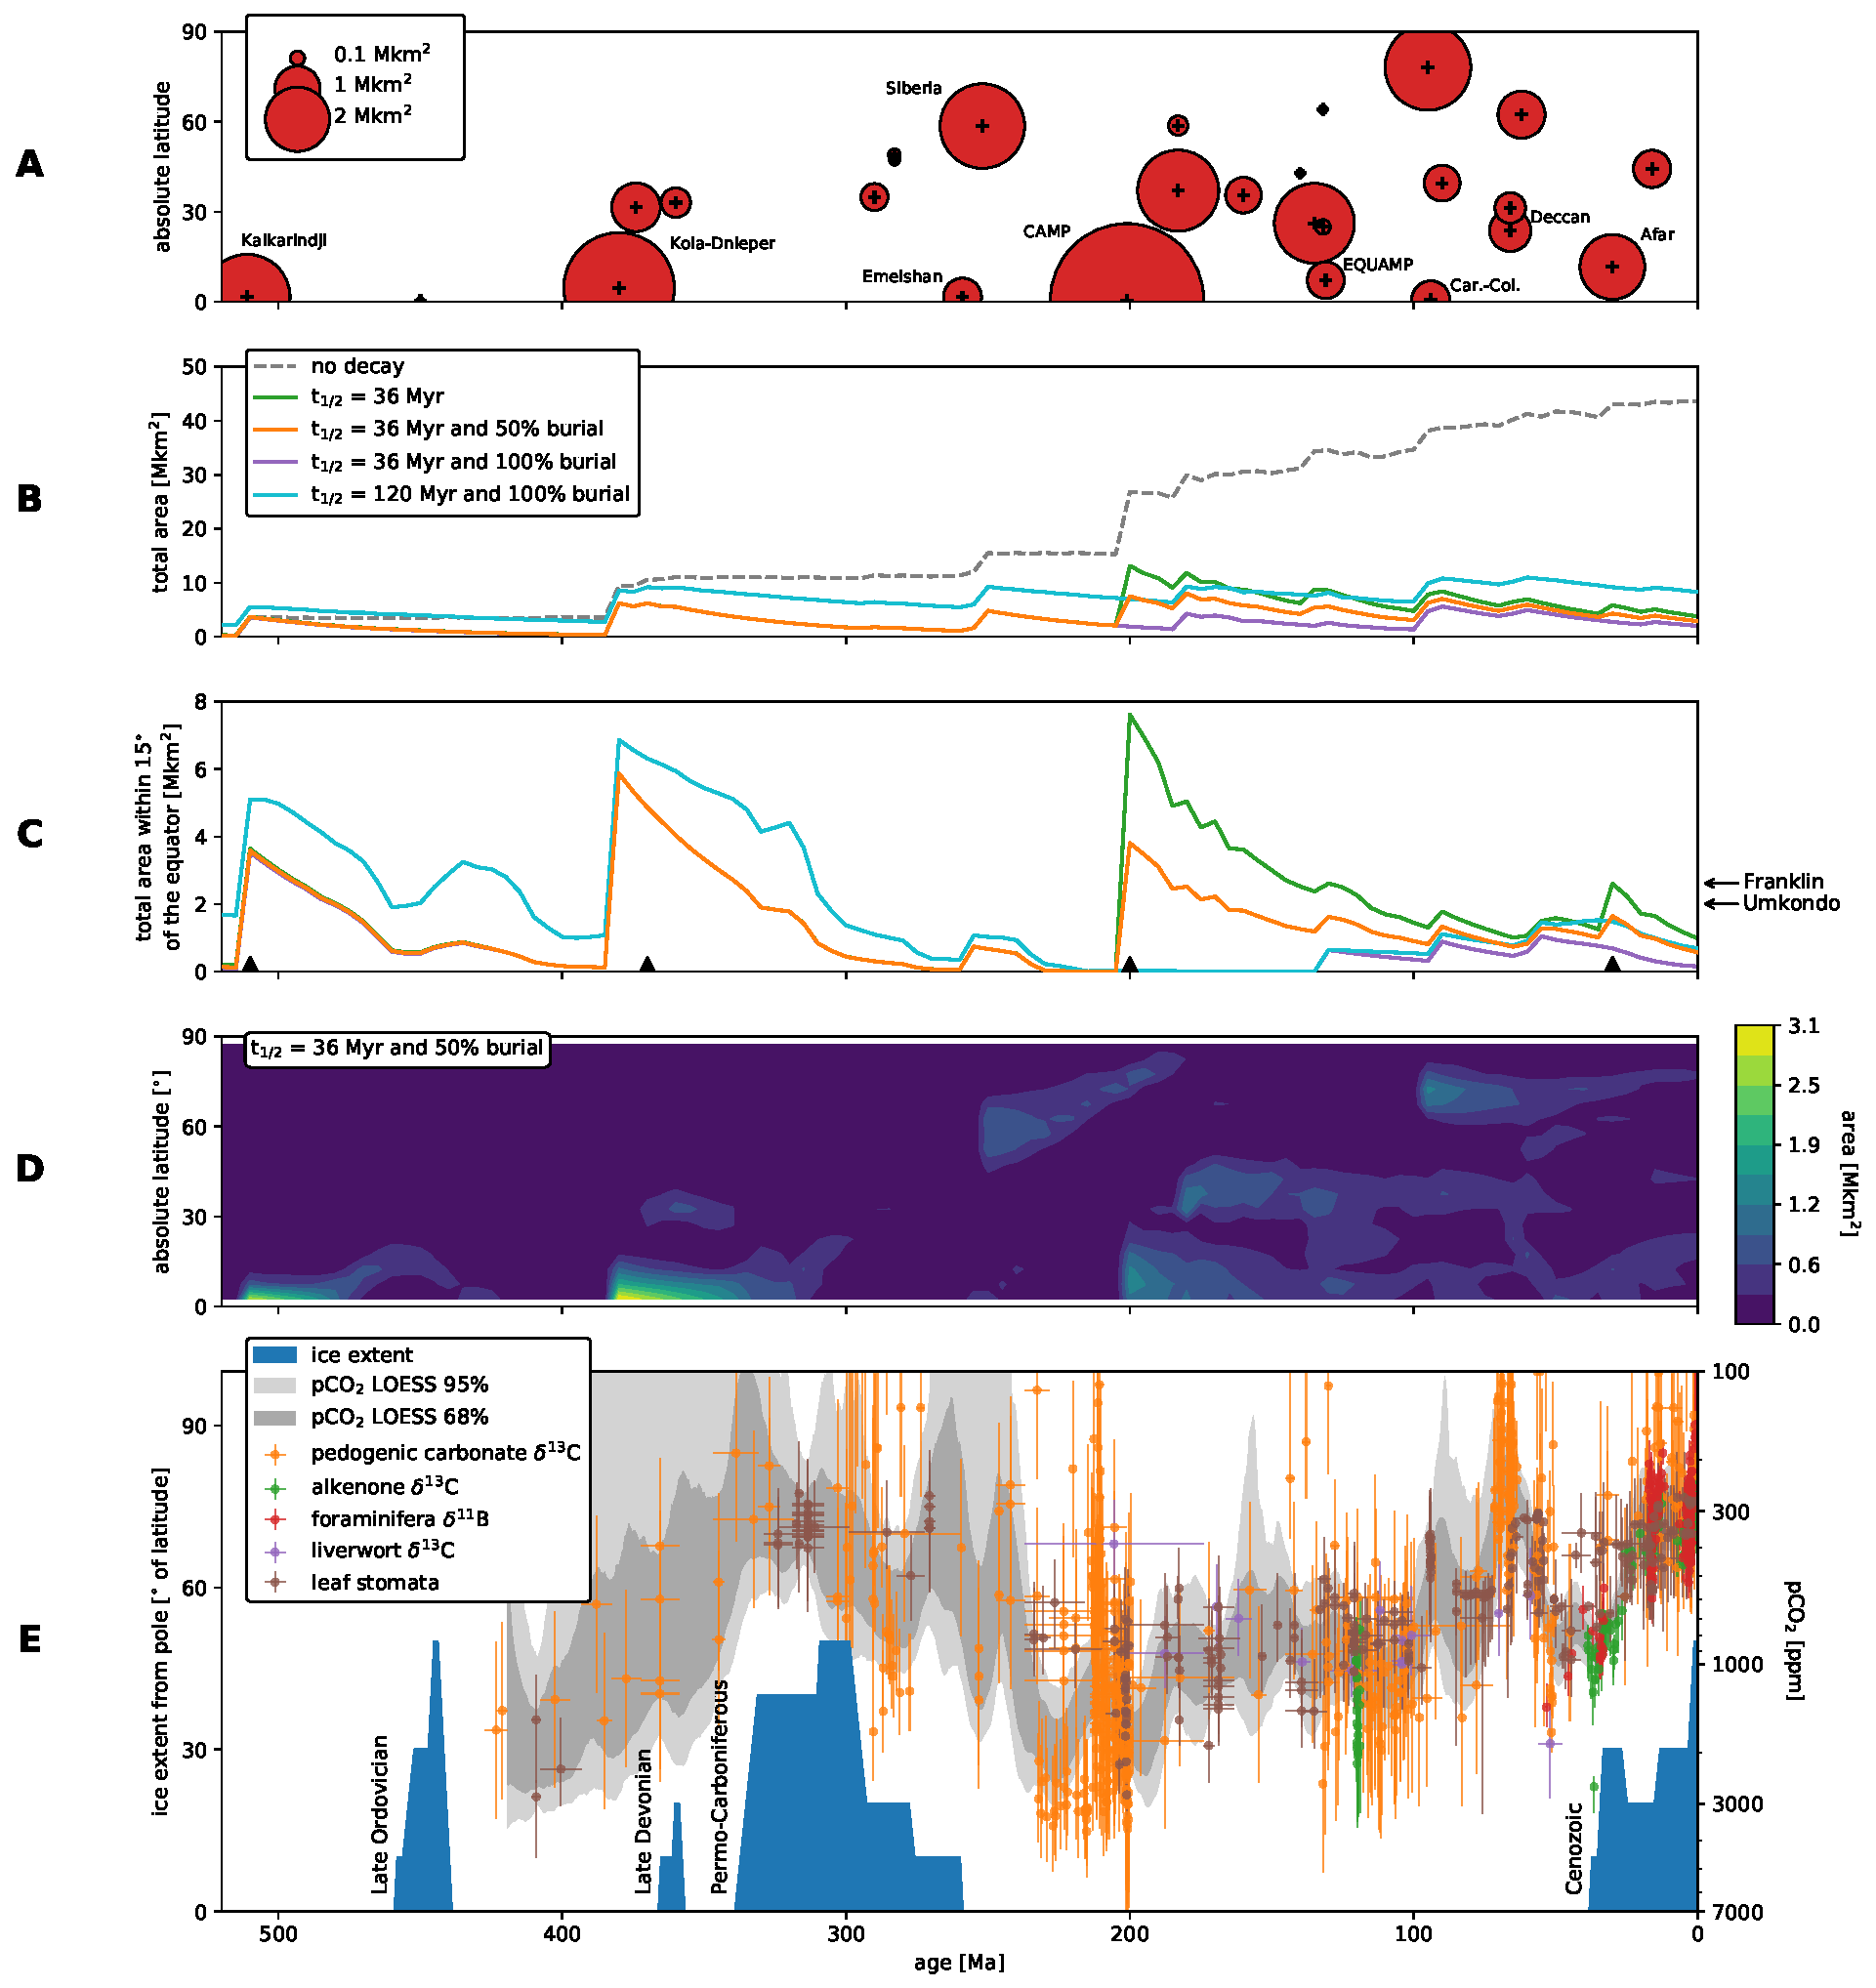
\includegraphics[width=0.9\textwidth]{./Manuscript/Figures/LIP_Areas.pdf}
	\caption{\textbf{A)} LIPs included in this analysis. The size of each circle reflects the initial surface area estimate of each LIP. The + indicates the timing and absolute paleolatitude of the centroid of each LIP at the time of emplacement. Car.-Col. = Caribbean-Colombian. \textbf{B)} Total LIP area through time for the different post-emplacent scenarios. Only the `no decay' scenario excludes pre-Phanerozoic LIPs. \textbf{C)} Tropical LIP area through time for the different post-emplacement scenarios. The arrows to the right indicate reconstructed tropical LIP area at the time of emplacement for the ca. 720 and 1109~Ma Franklin and Umkondo LIPs. The triangles show the paleogeographic reconstruction times in Fig. \ref{fig:Reconstruction_Snapshots}. \textbf{D)} Contour plot showing the latitudinal distribution of LIP area for one of the post-emplacement models. \textbf{E)} Latitudinal extent of land ice away from the poles \citep{Macdonald2019a} and compilation of \textit{p}CO$_{2}$ proxies \citep{Foster2017a} (\textit{p}CO$_{2}$ y-axis reversed, and in log-scale). Error bars indicate standardized uncertainties, and grey bands indicate 68 and 95\% confidence intervals for Monte Carlo resampled LOESS fits to the \textit{p}CO$_{2}$ proxy data \citep{Foster2017a}. Note that there are \textit{p}CO$_{2}$ proxy estimates \textless100~ppm that are cut off in this plot.}
	\label{fig:LIP_Areas}
\end{center}
\end{figure}

\begin{figure}[h!]
\begin{center}
	\includegraphics[width=\textwidth]{./Manuscript/Figures/Reconstruction_Snapshots.pdf}
	\caption{Paleogeographic reconstructions for times that correspond to peaks of LIP area in the tropics (Fig. \ref{fig:LIP_Areas}C). The opacity of LIP polygons indicates their parameterized remaining area at the time of the reconstruction as a percentage of initial LIP area, under the preferred post-emplacement scenario of `t$_{1/2}$ = 36~Myr + 50\% burial'.}
	\label{fig:Reconstruction_Snapshots}
\end{center}
\end{figure}

\begin{figure}[h!]
\begin{center}
	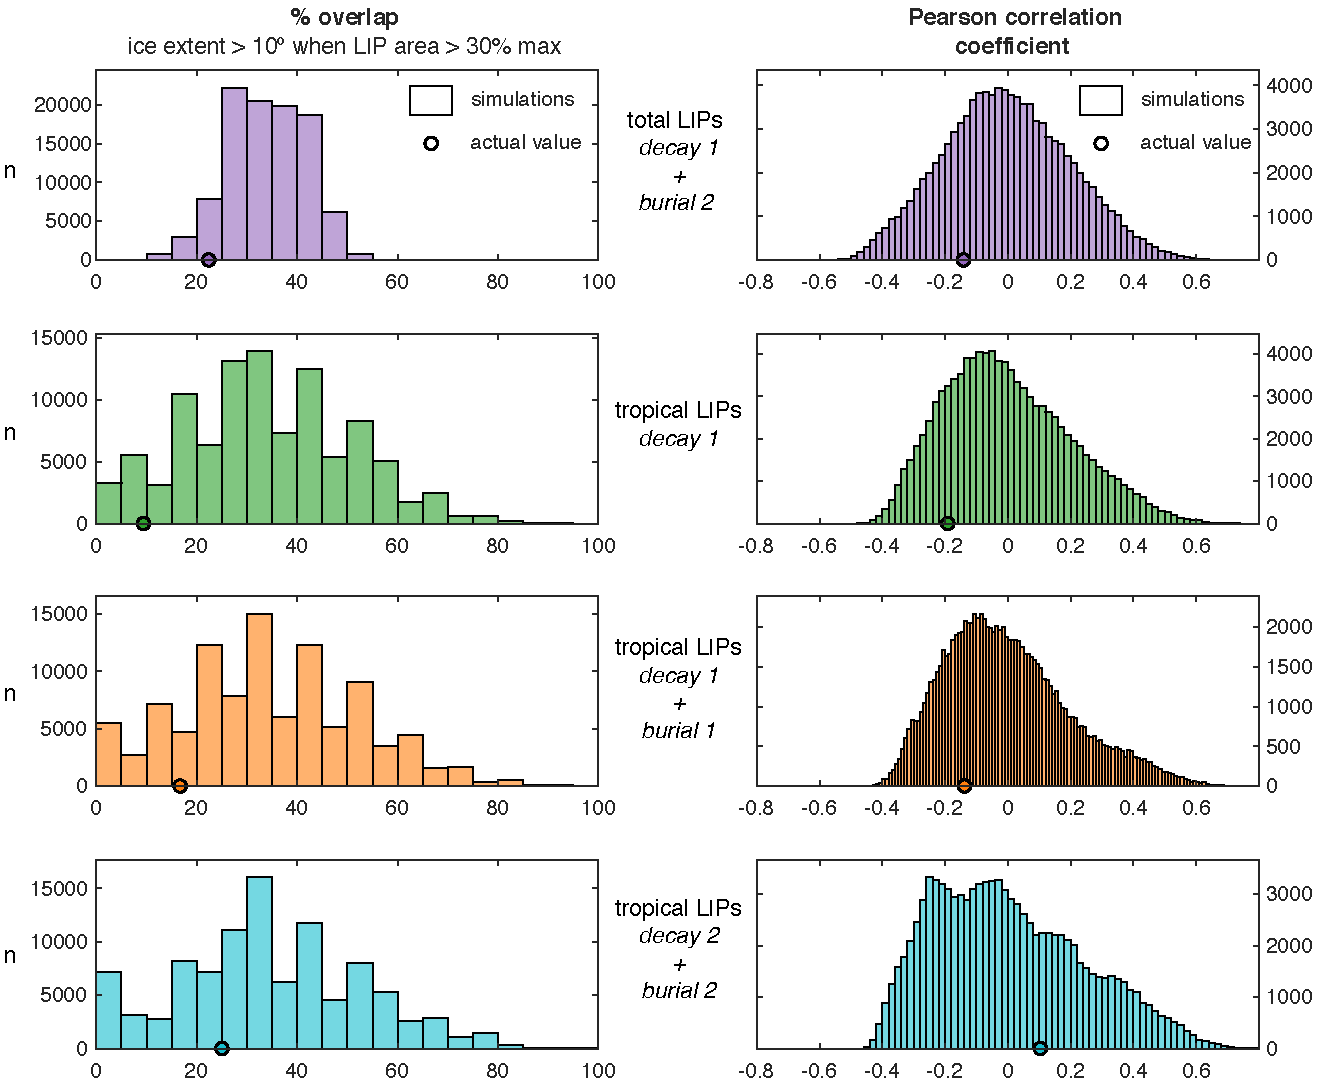
\includegraphics[width=0.85\textwidth]{./Manuscript/Figures/overlap_correlation_cropped.pdf}
	\caption{The \% overlap and Pearson correlation coefficients between LIP area and the actual ice-extent record are shown with circles. These values are compared to histograms that show the range of values that arise when comparing the LIP area record to glacial intervals that have been shifted randomly in time 100,000 times. The fraction of randomly timed glacial interval simulations that correlate/overlap better with LIP area than the actual ice-extent record is the p-value shown in Table \ref{tab:stats}.}
	\label{fig:LIP_correlation}
\end{center}
\end{figure}

\begin{figure}[h!]
\begin{center}
	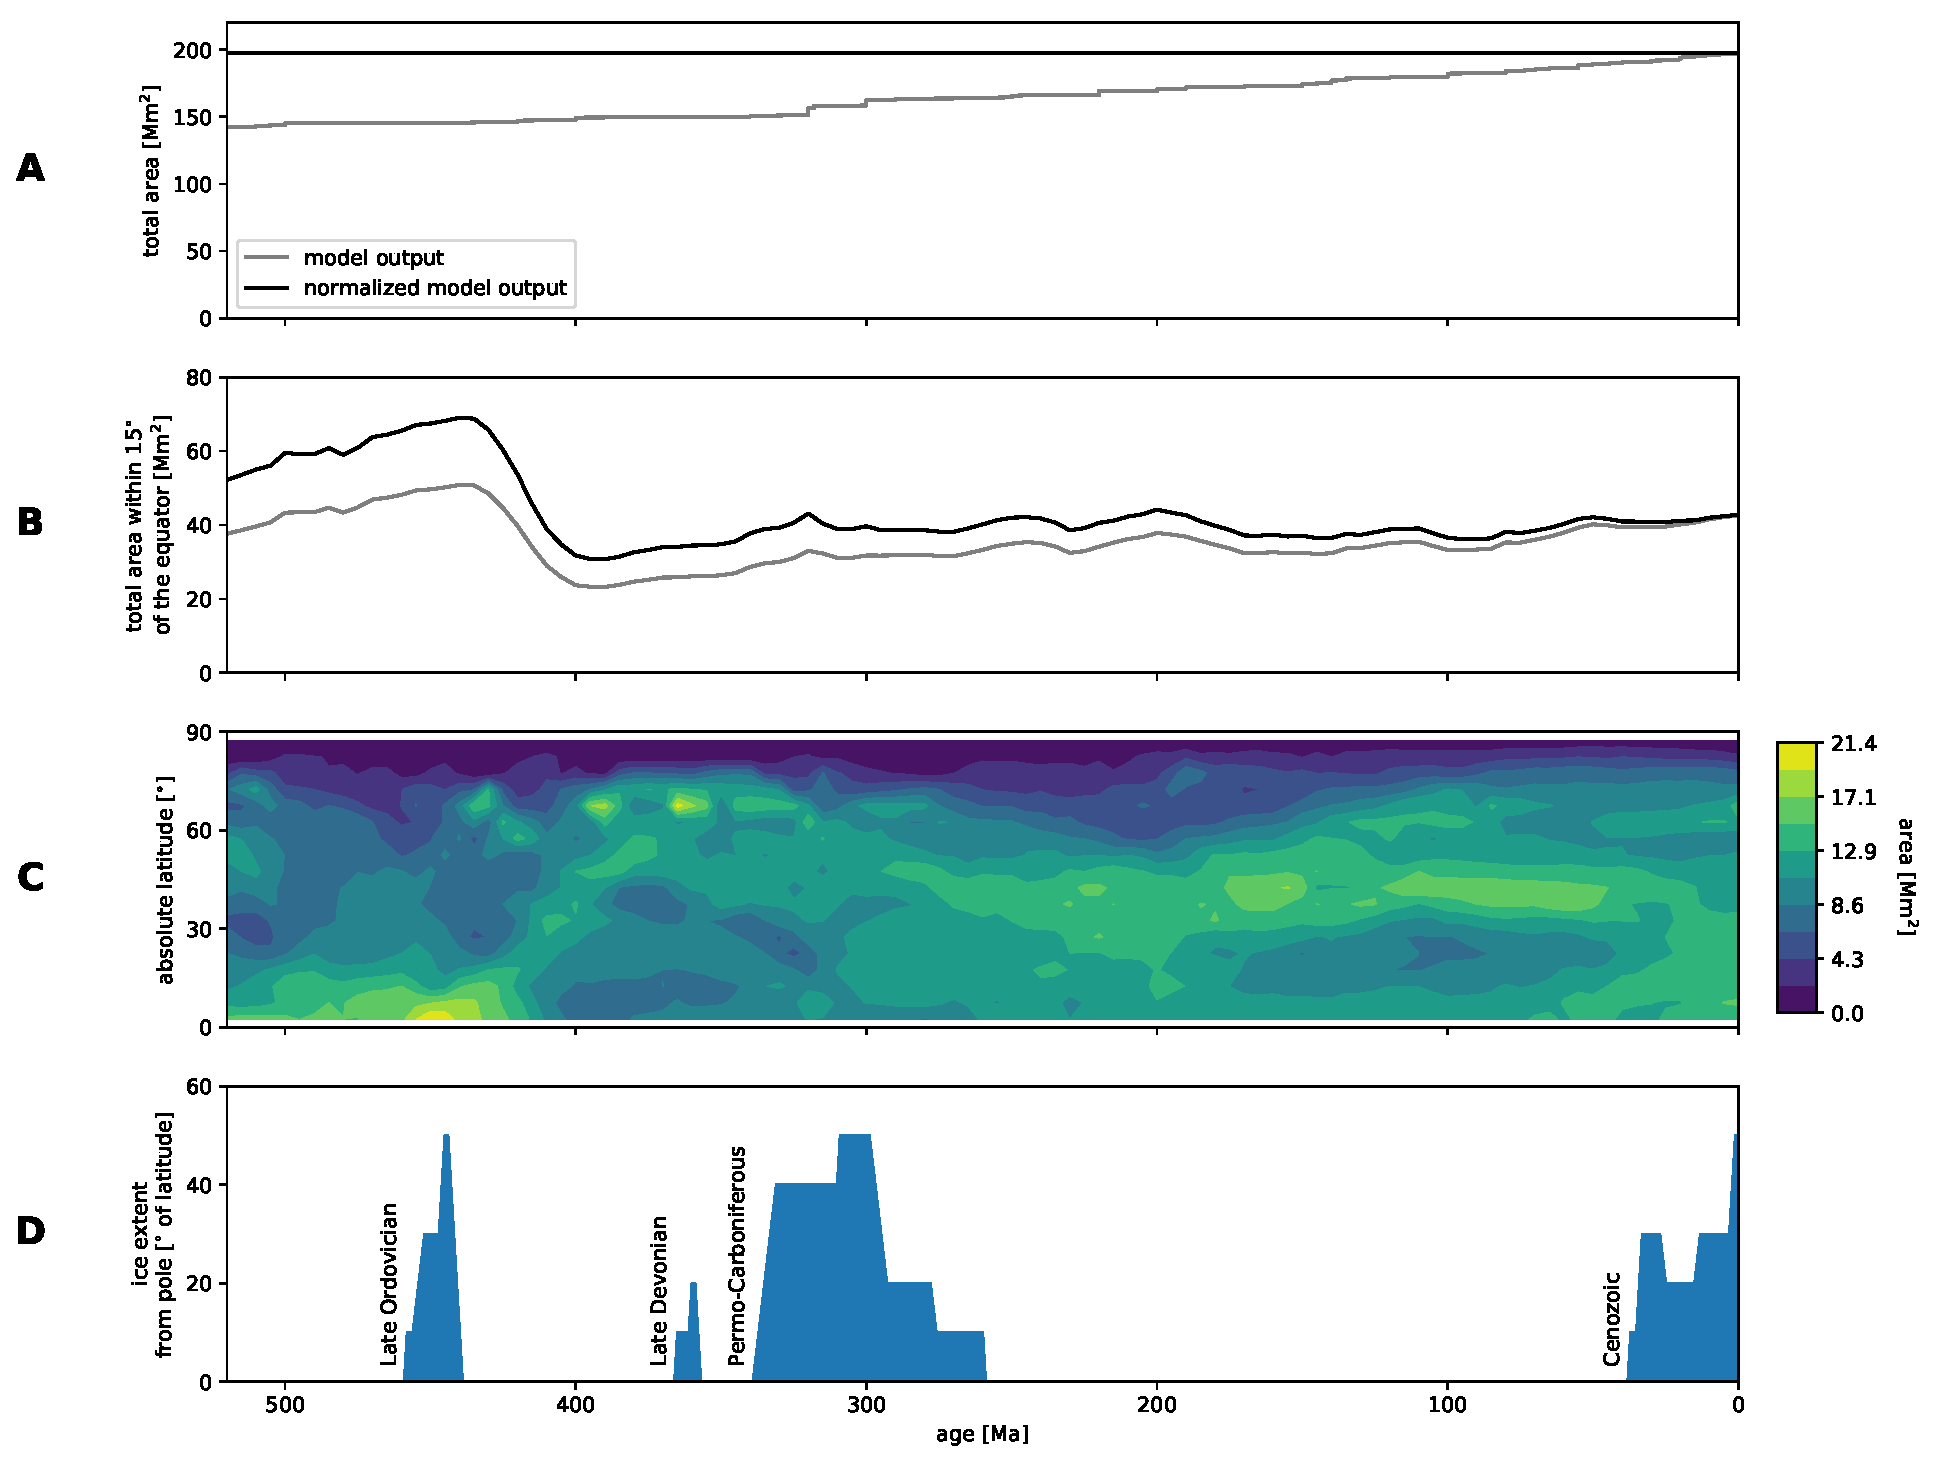
\includegraphics[width=0.9\textwidth]{./Manuscript/Figures/Continent_Areas.pdf}
	\caption{\textbf{A)} Total continental area through time. In the paleogeographic model used in this study, tectonic units \citep{Torsvik2016a} are progressively added to the model, leading to a net increase in total continental area in the model of $\sim$33\% over the Phanerozoic. However, estimates of continental crust growth (e.g. \citealp{Pujol2013a}) suggest that continental area was roughly constant through the Phanerozoic. We therefore normalize the total continental area curve in our model by assuming a fixed continental area through the Phanerozoic. \textbf{B)} Tropical continental area through time. We normalize the tropical continental area curve using the normalization ratio implied in (A). \textbf{C)} Contour plot showing the latitudinal distribution of continental area. \textbf{D)} Latitudinal extent of land ice away from the poles \citep{Macdonald2019a}.}
	\label{fig:Continent_Areas}
\end{center}
\end{figure}

\clearpage
\newpage
\footnotesize

\singlespacing

\bibliographystyle{./Manuscript/gsabull.bst}
\bibliography{./Manuscript/References.bib}

\nolinenumbers
\printindex

\end{document}
